\chapter{SoC 设计}

\section{概况}

为了更好地利用实验板提供的硬件资源,对 NonTrivialMIPS 进行功能演示,我们搭建了一个较为完整的 SoC,能够在大赛提供的实验箱上运行。

\subsection{SoC结构}

\begin{figure}[htbp]
    \centering
    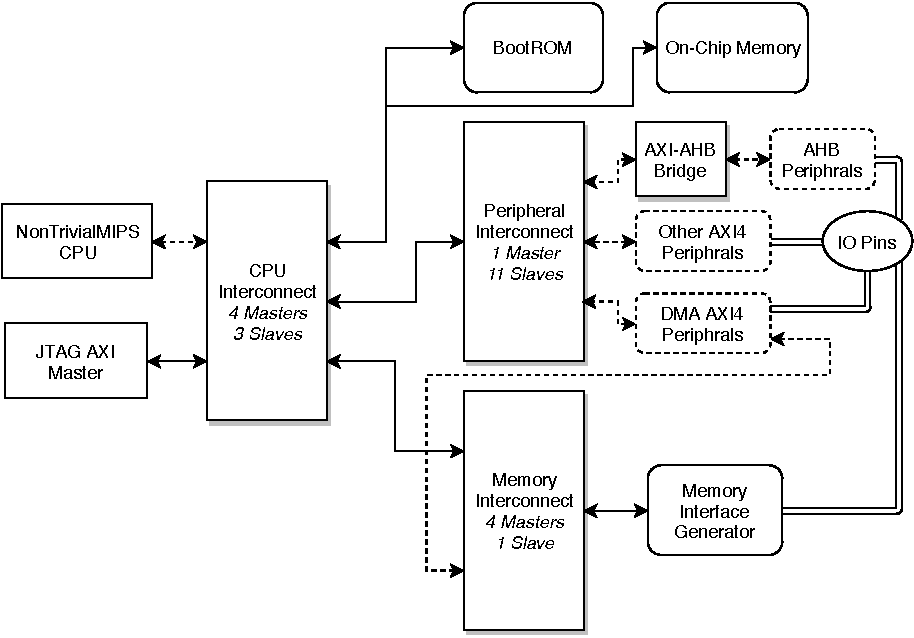
\includegraphics[width=\linewidth]{soc-structure.pdf}
    \caption{SoC结构}
    \label{fig:soc-structure}
\end{figure}

SoC由 Vivao 的 Block Design 设计功能组件,项目文件为 \texttt{vivado/NonTrivialMIPS.xpr},总体结构如图 \ref{fig:soc-structure} 所示。其中各个组件之间均使用标准的 AXI4 总线协议进行连接,并使用了多个 AXI Interconnect。图中无阴影的矩形表示 AXI Master,带阴影的矩形表示 AXI 总线互联(Interconnect)或适配器(Bridge),圆角矩形表示外设。图中的所有实线表示其为具体设备(及其连接关系),虚线表示由多个具体设备构成的一类设备(及其连接关系),双线表示到 FPGA 片外的连接。

我们将 NonTrivialMIPS CPU 的三个 AXI 接口(指令 Cache、数据 Cache、无 Cache 直通)直接连接到 CPU 互联模块上,不再需要预赛时 CPU 内部的互联模块。这一互联模块上还连接了 Xilinx 提供的 JTAG AXI Master IP,可以绕过 CPU 直接与设备进行通信,方便进行调试。这一互联模块直接连接了 BootROM 与片上 RAM(OCM) 两个使用 FPGA 的 Block RAM 资源生成的存储,以及外设互联、内存互联模块。这一设计使得 TrivialBootloader 等程序可以无需运行在内存中,而是在 OCM 中分配堆栈资源。这样,它就可以在内存的任意位置加载操作系统,而不用担心自身代码或数据被覆盖;并且当系统发生不可逆转或者没有捕获的异常/错误时,其依旧可以获取系统控制权,输出必要的调试信息后安全地停止工作。

外设互联模块上连接了除 DDR 内存控制器外所有的外设,其中由于部分外设使用 AHB 协议,我们额外连接了一个 AXI 到 AHB 协议的转换桥。

内存互联模块只有一个从设备,即 Xilinx 的 Mmemory Generator Interface IP 模块。在正确配置后,其能自动对板载的 DDR3 SDRAM 进行训练等操作,并将自己暴露为一片连续的存储空间供用户使用,隐藏了所有实现细节。除 CPU 互联模块外,内存互联的主设备还包含所有有 DMA 需求的外设,包括 VGA 控制器、FrameBuffer 读写控制器等。这样的连接能够让硬件在空闲时直接对内存进行读写,而无需 CPU 干预,大大加速了图形渲染、内存修改等过程。

\subsection{地址分配}

表 \ref{table:address_allocation} 列举了各个设备的物理地址空间分配,其对于总线上的所有 Master 设备都是一致的。

\begin{table}[!htbp]
    \centering
    \caption{外设物理地址分配}
    \label{table:address_allocation}
    \begin{tabular}{|c|c|c|c|c|}
    \hline
    \textbf{名称} & \textbf{起始地址} & \textbf{结束地址} & \textbf{有效大小} & \textbf{类型} \\ \hline
    DDR 控制器        & 0x00000000    & 0x07FFFFFF    & 128 MB          & 存储          \\ \hline
    OCM 控制器       & 0x08000000    & 0x0800FFFF    & 64 KB          & 存储          \\ \hline
    CFG Flash 控制器(内存映射) & 0x1A000000    & 0x1AFFFFFF    & 16 MB          & 存储          \\ \hline
    以太网控制器    & 0x1C000000    & 0x1C00FFFF    & 64 KB      & 寄存器          \\ \hline
    VGA 控制器        & 0x1C010000    & 0x1C01FFFF    & 64 KB         & 寄存器         \\ \hline
    PS/2 控制器        & 0x1C020000    & 0x1C020FFF    & 4 KB         & 寄存器         \\ \hline
    LCD 控制器        & 0x1C030000    & 0x1C030FFF    & 4 KB         & 寄存器         \\ \hline
    SPI Flash 控制器        & 0x1C040000    & 0x1C040FFF    & 4 KB         & 寄存器         \\ \hline
    USB 控制器        & 0x1C050000    & 0x1C050FFF    & 4 KB         & 寄存器         \\ \hline
    Framebuffer Reader 控制器        & 0x1C060000    & 0x1C06FFFF    & 64 KB         & 寄存器         \\ \hline
    Framebuffer Writer 控制器        & 0x1C070000    & 0x1C07FFFF    & 64 KB         & 寄存器         \\ \hline
    外部中断控制器        & 0x1D000000    & 0x1D00FFFF    & 64 KB         & 寄存器         \\ \hline
    BootROM 控制器       & 0x1FC00000    & 0x1FC1FFFF    & 128 KB          & 存储          \\ \hline
    串口控制器       & 0x1FD02000    & 0x1FD03FFF    & 8 KB          & 寄存器          \\ \hline
    GPIO 控制器       & 0x1FF00000    & 0x1FF0FFFF    & 64 KB          & 寄存器          \\ \hline

    \end{tabular}
\end{table}

\subsection{中断连接}

一些外设需要通过中断告知 CPU 自身的状态而完成 IO 操作。MIPS 规范中 CPU 至多支持 5 个外部中断(编号为 2 到 6),并且 NonTrivialMIPS 只支持电平触发的中断。因此,我们使用了 Xilinx Interrupt Controller IP 来对类型不同或者超出数量限制的中断进行统一转换和管理。表 \ref{table:interrupt-connection} 描述了这些中断的连接关系。

\begin{table}[!htbp]
    \centering
    \caption{中断连接关系}
    \label{table:interrupt-connection}
    \begin{tabular}{|c|c|c|c|}
    \hline
    \textbf{名称} &  \textbf{中断类型} & \textbf{接收方} & \textbf{中断编号} \\ \hline
    串口控制器       & 高电平    & CPU     & 2          \\ \hline
    PS/2 控制器       & 高电平    & CPU     & 3          \\ \hline
    AXI 中断控制器       & 高电平    & CPU     & 6          \\ \hline
    以太网控制器       & 上升沿    & AXI中断控制器     & 0          \\ \hline
    SPI Flash 控制器       & 上升沿    & AXI中断控制器     & 1          \\ \hline
    CFG Flash 控制器       & 上升沿    & AXI中断控制器     & 2          \\ \hline
    USB 控制器       & 高电平    & AXI中断控制器     & 3          \\ \hline
    \end{tabular}
\end{table}

\section{硬件支持}

FPGA 板载了较多的物理接口和硬件资源,为了充分利用,达到较好的展示效果,我们均对它们进行了适配。

\subsection{串口控制器}

板载串口为 RS-232 接口,我们使用 Xilinx 提供的 AXI UART 16550 IP 实现了一个标准的 NS16550 UART 控制器。其支持比较完整的串口协议,包括可变波特率、流量控制和读写缓冲区。在软件使用串口前,需要首先对多个配置寄存器进行初始化,配置波特率、中断等不同的属性,方可正常与 PC 进行通信。串口控制器有一个中断,指示收到了数据,它被直接连接到 CPU 的第一个硬件中断上。

\subsection{USB 控制器}

实验箱上的 USB PHY 为 Microchip USB 3500 ,支持 Host/Device/OTG 三种模式下的 USB 2.0 协议。它提供的是 UTMI+ Level 3.0 的接口,我们从实验箱的原理图中找到了对应引脚在 FPGA 上的绑定,并添加到约束文件中。由于 USB 3500 仅实现了物理层的收发逻辑,我们以开源的 UltraEmbedded USB 1.1 Host Controller IP 为基础,进行了大量的修改以满足使用需求。具体工作将工作频率调整为 USB 2.0 Full Speed 指定的 60MHz、调整 IFS 逻辑、添加输出延迟约束等等。此外,我们也需要移植驱动到 U-Boot 和Linux 中,这将在下面的系统软件部分中详述。

\subsection{以太网控制器}USB

实验箱上提供了一个 10/100 Mbps 的以太网 PHY (物理接口),引出了以太网协议中规定的标准的 MII 和 MDIO 接口,用于数据传输和物理芯片配置。我们使用了 Xilinx 提供的 AXI Ethernet Lite IP 实现以太网控制器,在 U-Boot 和 Linux 中都有对应的驱动。这一控制器不支持 DMA,因此实际的数据传输无法达到 100 Mbps 全速工作。事实上,经过测试,速度最高可达到 2MB/s 左右,已经足够;考虑到内存带宽分配问题,我们没有使用完整的 Xilinx Ethernet MAC 和 DMA IP。由于该 IP 仅提供上升沿触发的中断,我们使用中断控制器来转换中断类型。

\subsection{Flash 控制器}

实验室上共有两片 SPI NOR Flash 芯片,其中一片固化连接至FPGA 配置专用硬件逻辑,另一片是普通 SPI I/O 引脚,可以插拔更换 Flash 芯片。我们都使用 Xilinx 提供的 AXI Quad SPI IP 来进行控制。

对于配置 Flash(即 CFG Flash),其主要作用是存储 FPGA 的 bitstream,在上电时自动对 FPGA 进行配置。其总容量为 16 MB,而 bitstream 只会占用 6到7 MB 的空间,因此我们在剩余空间中存储了 U-Boot 和 Linux Kernel 的 ELF 格式文件。为了方便地使用配置 Flash,通过 IP 的 XIP(Execute In Place)特性,我们可以将它映射为一块只读的内存空间,从而 TrivialBootloader 可以直接从中加载 U-Boot,U-Boot 也能加载 Linux 内核。

另一块可插拔的 Flash(称为 SPI Flash)被我们用作通用的存储,因此 XIP 的只读模式不能满足需求。我们将其暴露为一个标准的 SPI 控制器,由软件来进行相应的管理。U-Boot 与 Linux 都有 SPI 协议和 Flash 读写、MTD 设备支持。通过测试,我们能够正确地对 Flash 进行擦除、读取、写入等操作。同时,为了 IO 更高效,我们还将 IP 提供的中断引出,通过中断控制器连接到 CPU。

\subsection{LCD 控制器}

实验板板载了一块 NT35510 LCD 屏幕,分辨率为 $800 \times 480$。它事实上是一个通用的异步类 SRAM 设备,有一个指令寄存器和一个数据寄存器,可以通过信号控制,分别进行读写。我们使用了 Verilog 实现的 NT35510 控制器(感谢张宇翔同学早先的移植),将两个寄存器分别映射到两个地址,通过 APB 协议(转换后为 AXI 协议)即可控制屏幕。控制器只是实现了到屏幕的通信,其本身的控制逻辑比较复杂,我们会在下面的驱动移植部分中较为详细地叙述。

\subsection{VGA 控制器}

实验板提供了标准的 VGA 接口,我们使用 Xilinx 提供的 Thin Film Transistor Controller IP 来实现图象的输出。它事实上提供了一个标准的 Framebuffer,可以通过控制 AXI 信号写入起始地址等配置,而在被启动后,通过 DMA 的方法不断从内存中读取图像数据,转换为符合 VGA 时序的信号输出。其输出的图像分辨率固定为 $640 \times 480$,24 位真彩色。由于提供的 DAC 实际深度小于24位,我们将较低位舍弃,对图像质量没有明显影响。

由于 Framebuffer 将被 Linux 作为控制台和主视频输出使用,而使用过程中将频繁发生像素的拷贝(如窗口移动、终端滚屏等),因此我们添加了 Xilinx 的 Framebuffer Reader 和 Framebuffer Writer 这两个 IP,用 DMA 的方式完成内存的拷贝。在两者的 AXI Stream 协议之间,我们添加了一个简单的 RTL 模块,可以将途径其的像素数据替换为常数或者异或一个常数(这也是 Linux 经常进行的任务,用于绘制一个矩形或者阴影等)。这一硬件组件可用于加速 Framebuffer 的绘制,也需要 Linux 中相应软件驱动的配合,具体将在下面章节中说明。

\subsection{PS/2 控制器}

实验板载一个 PS/2 物理接口,可以用于连接较老的鼠标/键盘等设备。我们使用 Altera 提供的 University Program PS/2 IP 对其进行控制,在 Linux 中也有对应的驱动支持。由于其为 APB 总线,同样需要 Bridge 进行转换;它的中断信号被直接连接到 CPU 的 3 号中断引脚。

\subsection{GPIO 控制器}

实验班上还有较多的 GPIO 设备,包括拨码开关、案件、数码管、单双色 LED 等。由于龙芯提供的 \texttt{confreg} 模块已经较好地对这些外设进行了统一控制和管理,还提供了额外的计时器、虚拟串口等功能,并包装为 AXI 接口。考虑到没有必要进行重复的实现,我们直接使用了这一模块。需要注意的是,由于其硬编码了一些参数(包括一些信号宽度),需要进行一些修复,才能直接使用在 Block Design 中。
